%%%%%%%%%%%%%%%%%%%%%%%%%%%%%%%%%%%%%%%%%%%%%%%%%%%%%%%%%%%%%%
%% Rozdział 3: Platforma do anotacji
%%%%%%%%%%%%%%%%%%%%%%%%%%%%%%%%%%%%%%%%%%%%%%%%%%%%%%%%%%%%%%

\section{Platforma do anotacji}
\label{chap:annotation-platform}

Korpusy języka migowego odpowiednie do trenowania modeli opisanych
w rozdziałach~\ref{chap:isolated-gloss-recognition} i~\ref{chap:text-translation}
są nieliczne, co uzasadniało stworzenie dedykowanej platformy do gromadzenia
 i oznaczania nagrań wideo w języku migowym. W tym rozdziale opisano wymagania
funkcjonalne, architekturę systemu oraz format danych tej platformy. Kod źródłowy
platformy jest publicznie dostępny w serwisie GitHub pod adresem
\url{https://github.com/stachurski2k/SLEP}, gdzie znajduje się również tablica
projektowa wykorzystywana do zarządzania pracami.

\subsection{Wymagania funkcjonalne}
\label{sec:annotation-functional-requirements}

Główne cele prac programistycznych nad platformą do anotacji obejmowały:

\begin{itemize}
  \item stworzenie działającej aplikacji do gromadzenia zbiorów nagrań wideo
        w języku migowym;
  \item zapewnienie możliwości zarządzania zbiorami danych, nagraniami wideo,
        klasami gestów i typami gestów;
  \item obsługę przesyłania nagrań wideo z wykorzystaniem magazynu obiektowego
        zamiast przechowywania dużych plików bezpośrednio w bazie danych;
  \item asynchroniczne przetwarzanie przesłanych nagrań, tak aby ekstrakcja
        punktów charakterystycznych nie blokowała żądań HTTP;
  \item ekstrakcję punktów charakterystycznych ciała, twarzy i dłoni z nagrań
        wideo z wykorzystaniem MediaPipe;
  \item udostępnienie edytora przeglądarkowego do wybierania zakresów klatek
        i zapisywania anotowanych fragmentów nagrań z gestami;
  \item przygotowanie projektu do lokalnego rozwijania z wykorzystaniem
        Docker Compose.
\end{itemize}

Frontend zaimplementowano przy użyciu React~19, TypeScript, Vite, React Router,
Tailwind CSS, ESLint oraz biblioteki powiadomień Sonner. Interfejs wykorzystuje
ciemny motyw o profesjonalnym wyglądzie i jest zorganizowany wokół komponentów
wielokrotnego użytku, takich jak tabele, okna dialogowe, nawigacja i edytor wideo.
Frontend udostępnia kilka głównych widoków, obsługiwanych przez obszary API
wymienione w podrozdziale~\ref{sec:annotation-system-architecture}:

\begin{itemize}
  \item \textbf{Edytor wideo} -- umożliwia wybór zbiorów danych i nagrań,
        podgląd bieżącego nagrania, przechodzenie między klatkami, ustawianie
        początku i końca klipu, przypisywanie metadanych gestu oraz zapisywanie
        klipów. Wczytuje wybrane nagrania za pomocą podpisanych adresów URL
        do pobierania, wyświetla elementy sterowania odtwarzaniem, obsługuje
        nawigację klatka po klatce, pokazuje oś czasu z możliwością przybliżania,
        przechowuje znaczniki klatek początkowej i końcowej oraz przesyła anotacje
        klipów do backendu. Zapisuje również wybraną klasę i typ gestu w pamięci
        lokalnej przeglądarki, aby ograniczyć konieczność wielokrotnego ręcznego
        wybierania tych samych wartości podczas anotacji;
  \item \textbf{Menedżer zbiorów danych} -- umożliwia wyświetlanie listy zbiorów
        danych, tworzenie nowych zbiorów, usuwanie zbiorów oraz otwieranie widoku
        nagrań należących do wybranego zbioru;
  \item \textbf{Widok nagrań zbioru danych} -- umożliwia wyświetlanie listy
        nagrań należących do zbioru, podgląd wybranych nagrań, import nowych
        nagrań oraz otwieranie ich w edytorze;
  \item \textbf{Zarządzanie klasami gestów} -- umożliwia utrzymywanie listy
        klas gestów wykorzystywanych podczas anotacji;
  \item \textbf{Zarządzanie typami gestów} -- umożliwia utrzymywanie listy
        typów gestów wykorzystywanych podczas anotacji.
\end{itemize}

\begin{figure}[htbp]
  \centering
  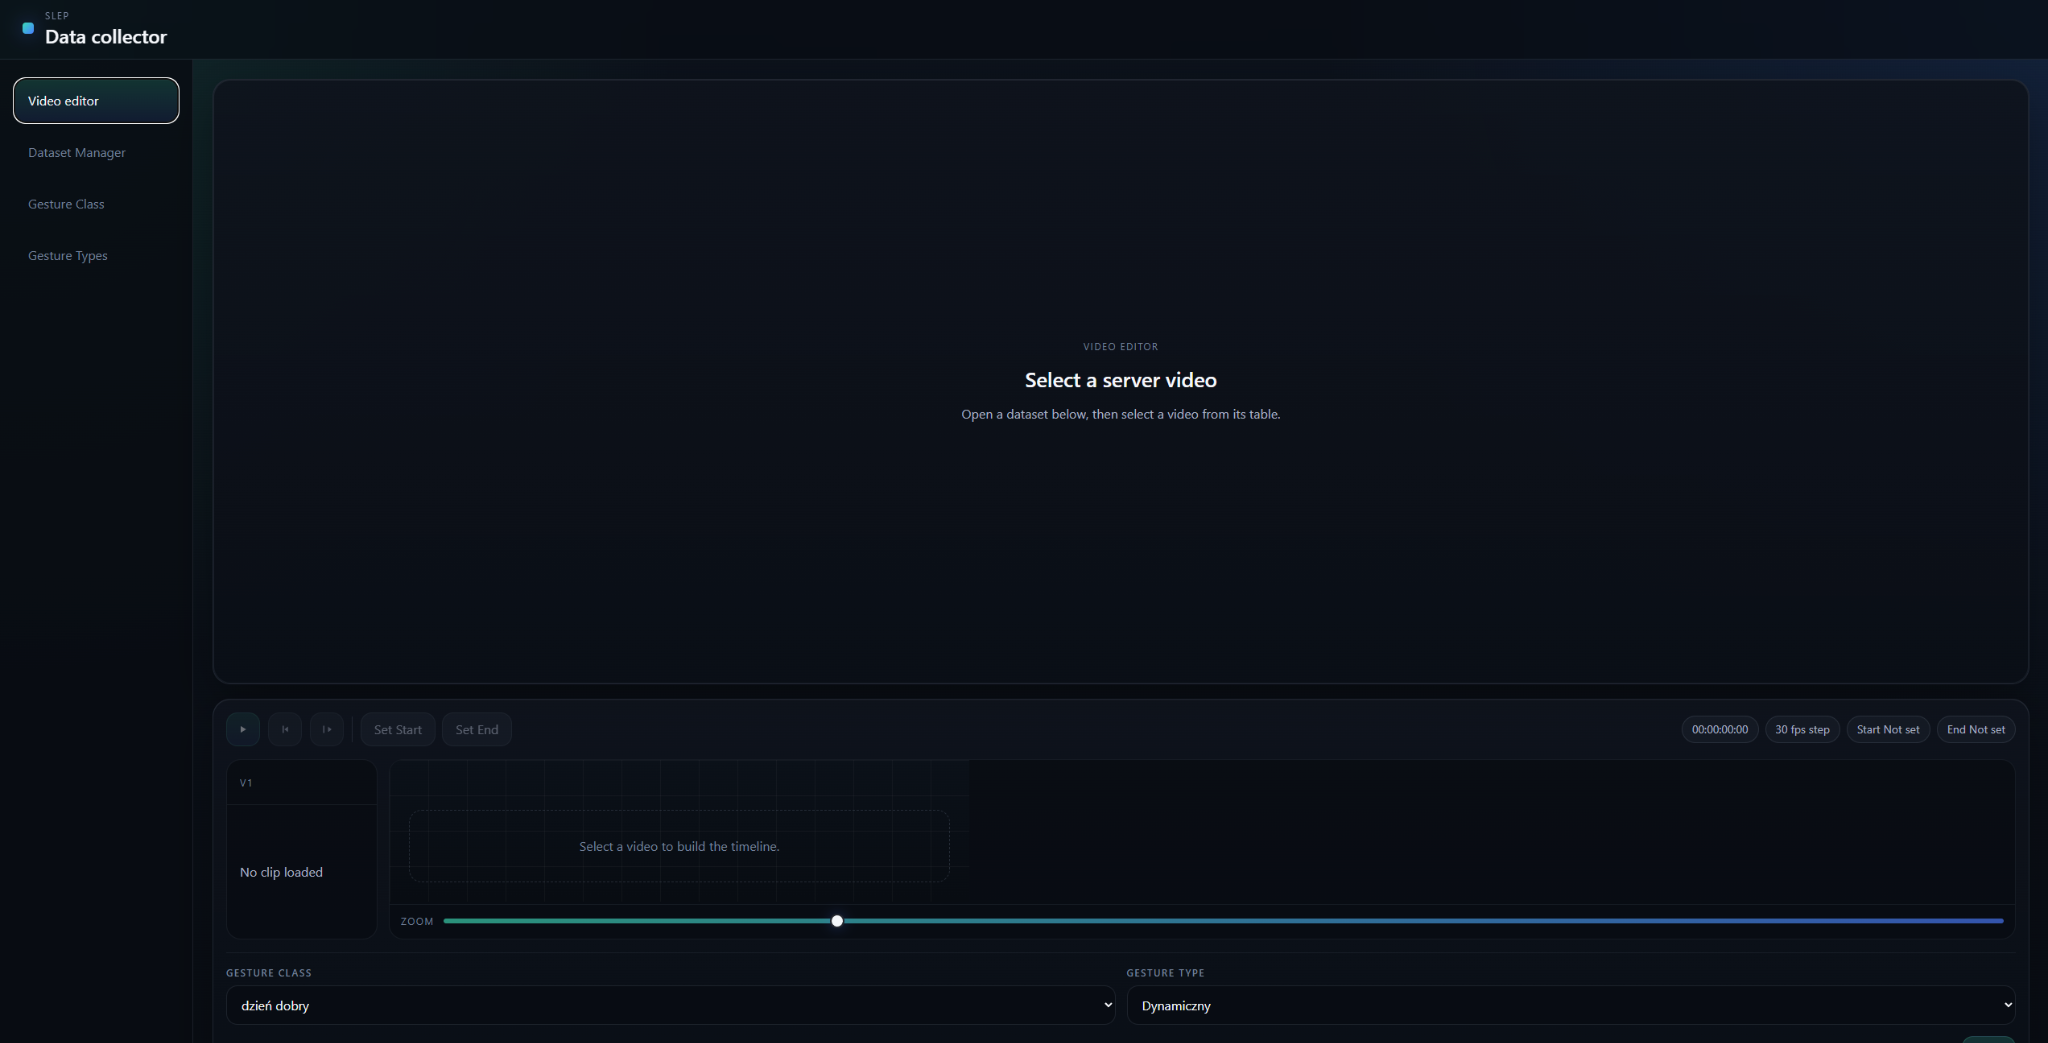
\includegraphics[width=0.85\textwidth]{figures/annotation-platform/video-editor-page.png}
  \caption{Widok edytora wideo.}
  \label{fig:video-editor-page}
\end{figure}

\begin{figure}[htbp]
  \centering
  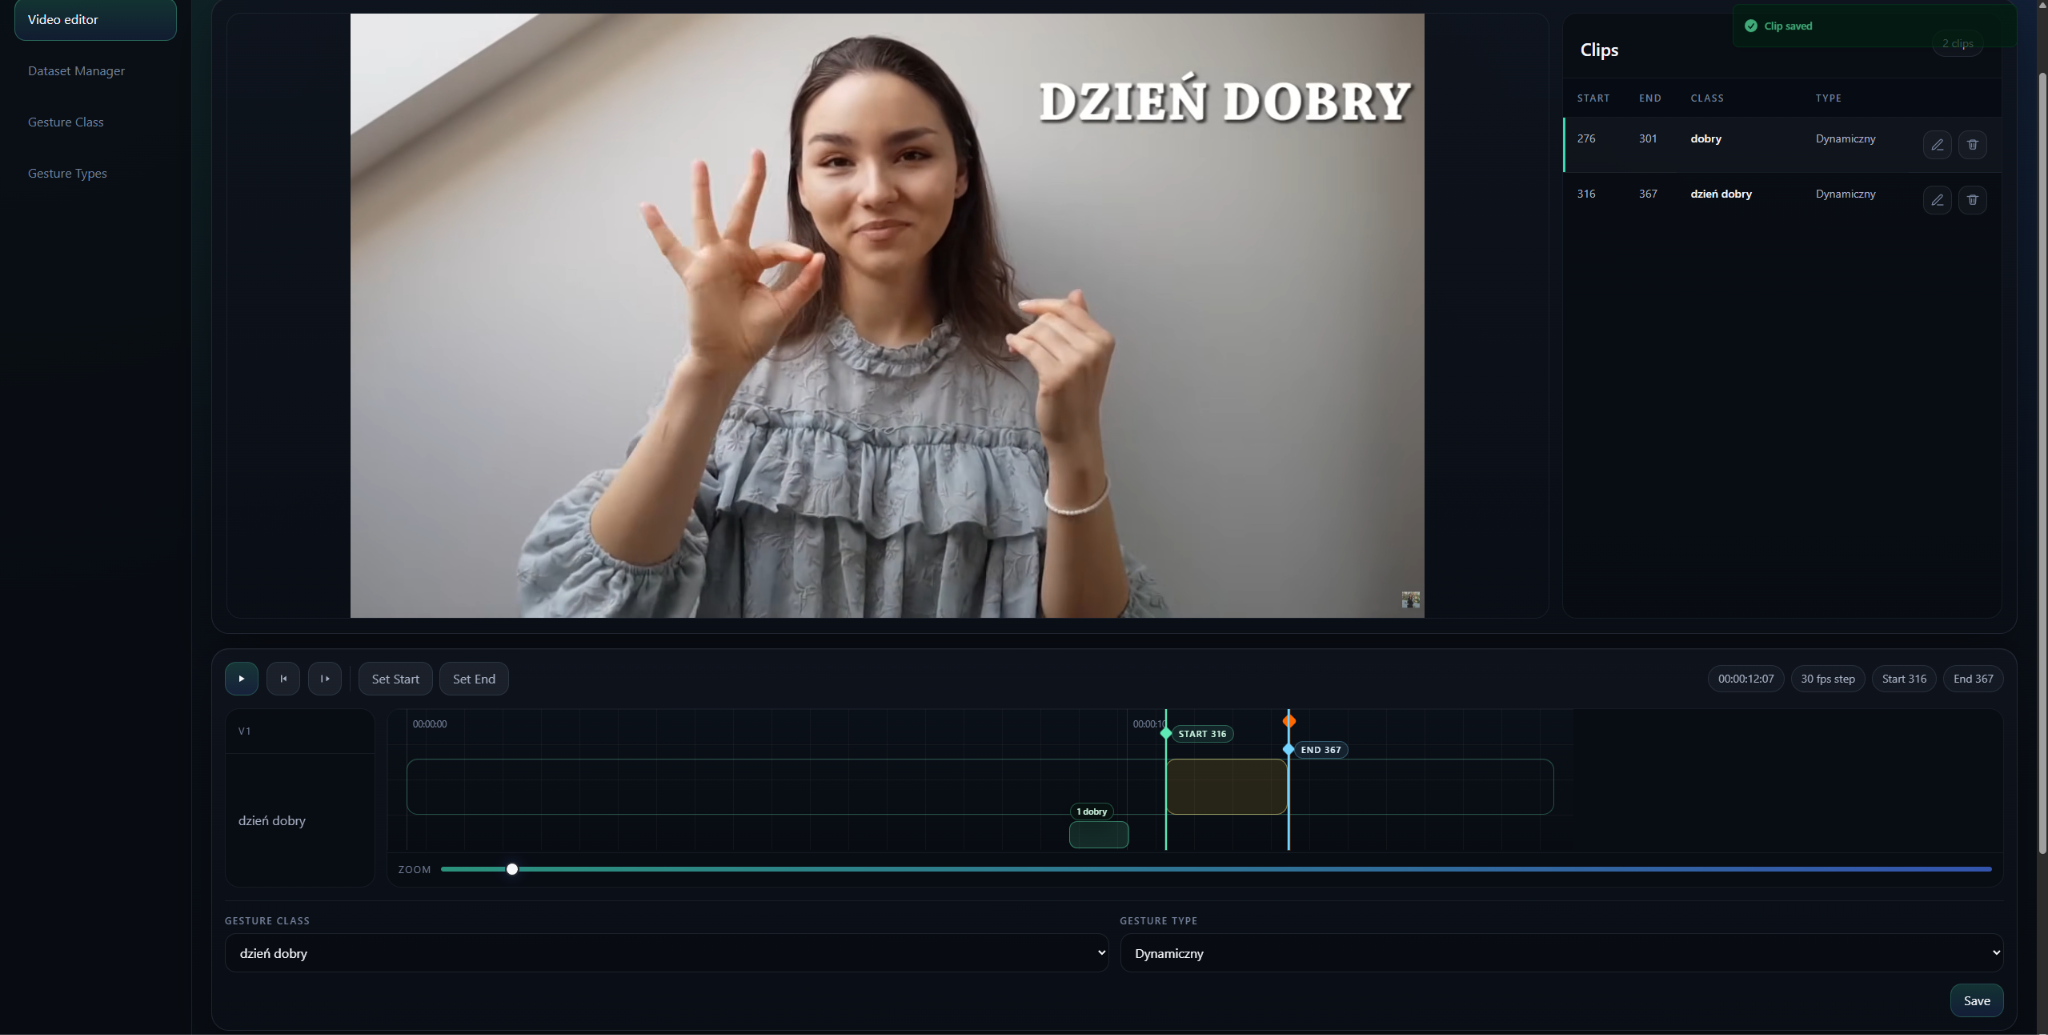
\includegraphics[width=0.85\textwidth]{figures/annotation-platform/video-editor-sample.png}
  \caption{Edytor wideo z wczytanym przykładowym nagraniem.}
  \label{fig:video-editor-sample}
\end{figure}

\begin{figure}[htbp]
  \centering
  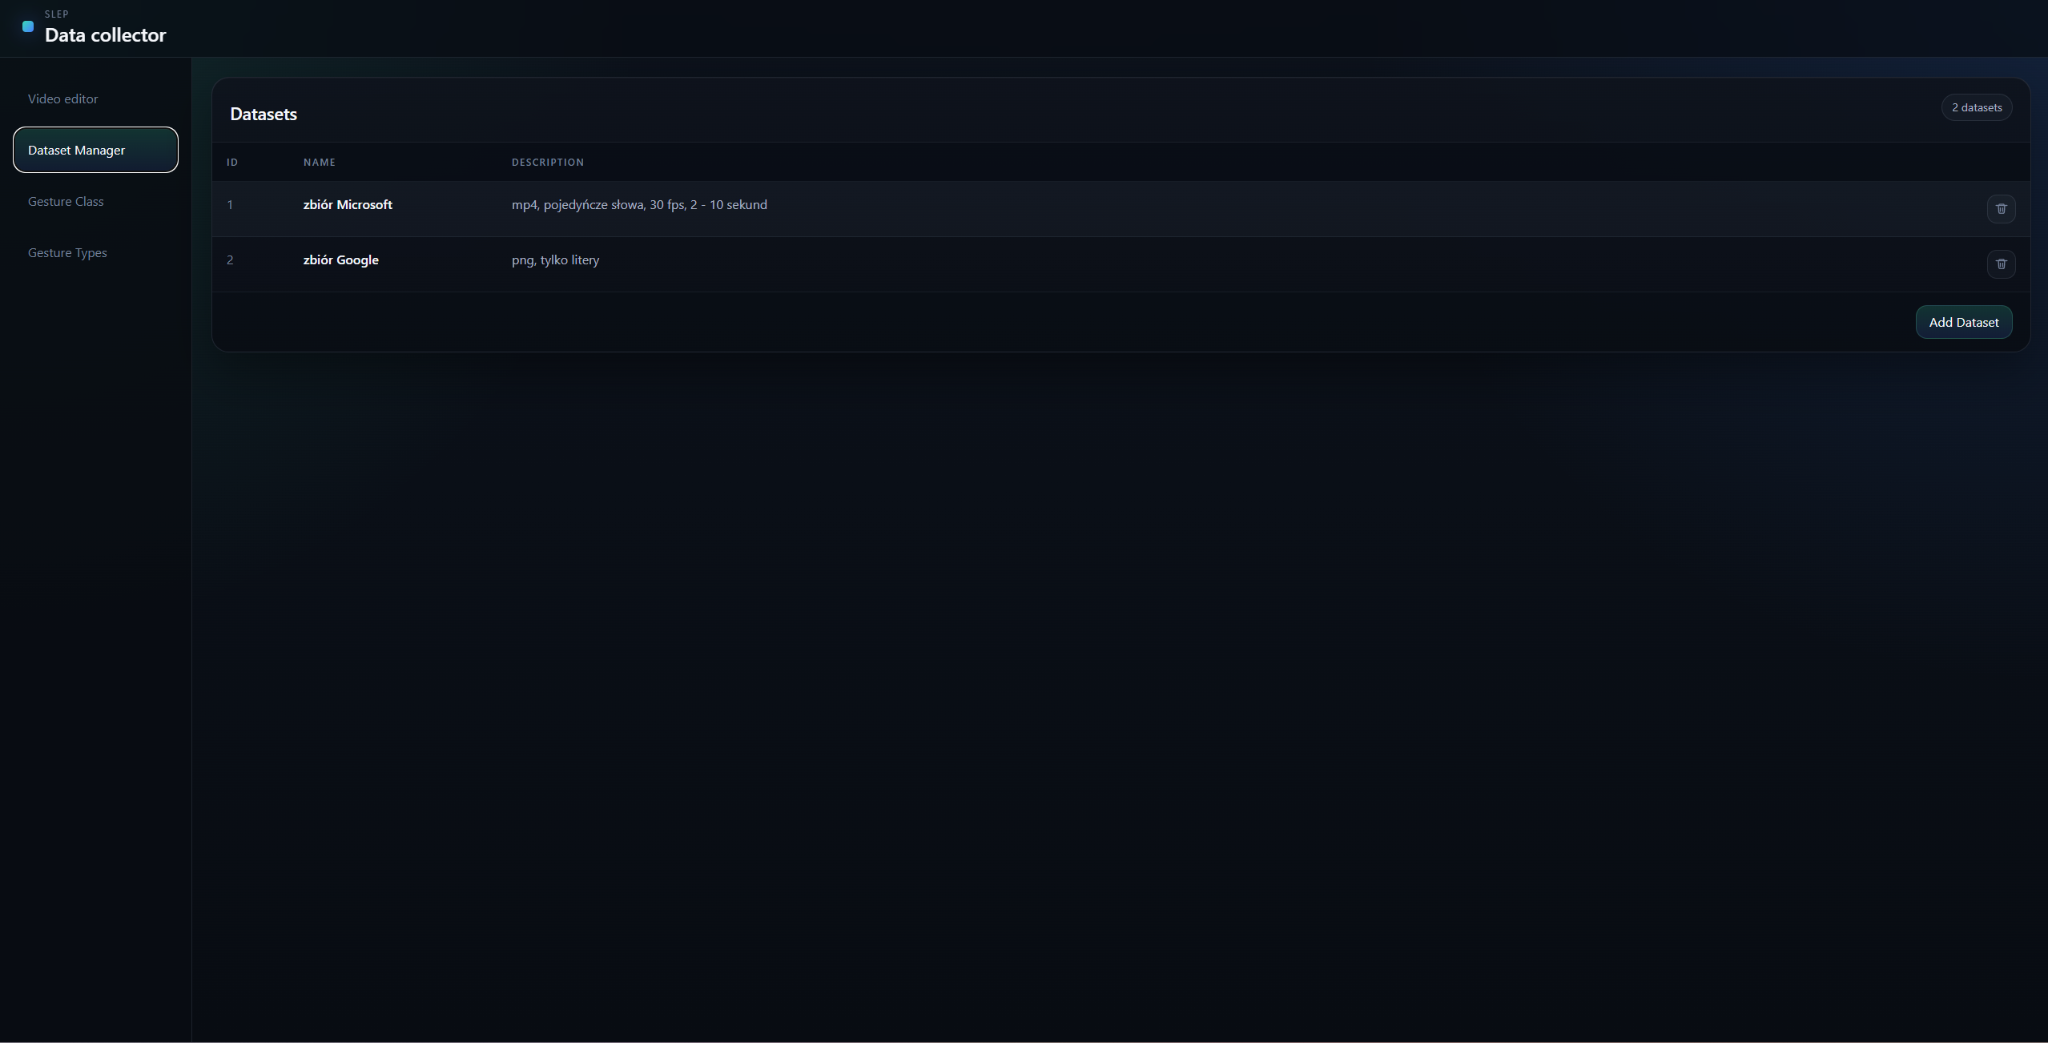
\includegraphics[width=0.7\textwidth]{figures/annotation-platform/dataset-manager-page.png}
  \caption{Widok menedżera zbiorów danych.}
  \label{fig:dataset-manager-page}
\end{figure}

\begin{figure}[htbp]
  \centering
  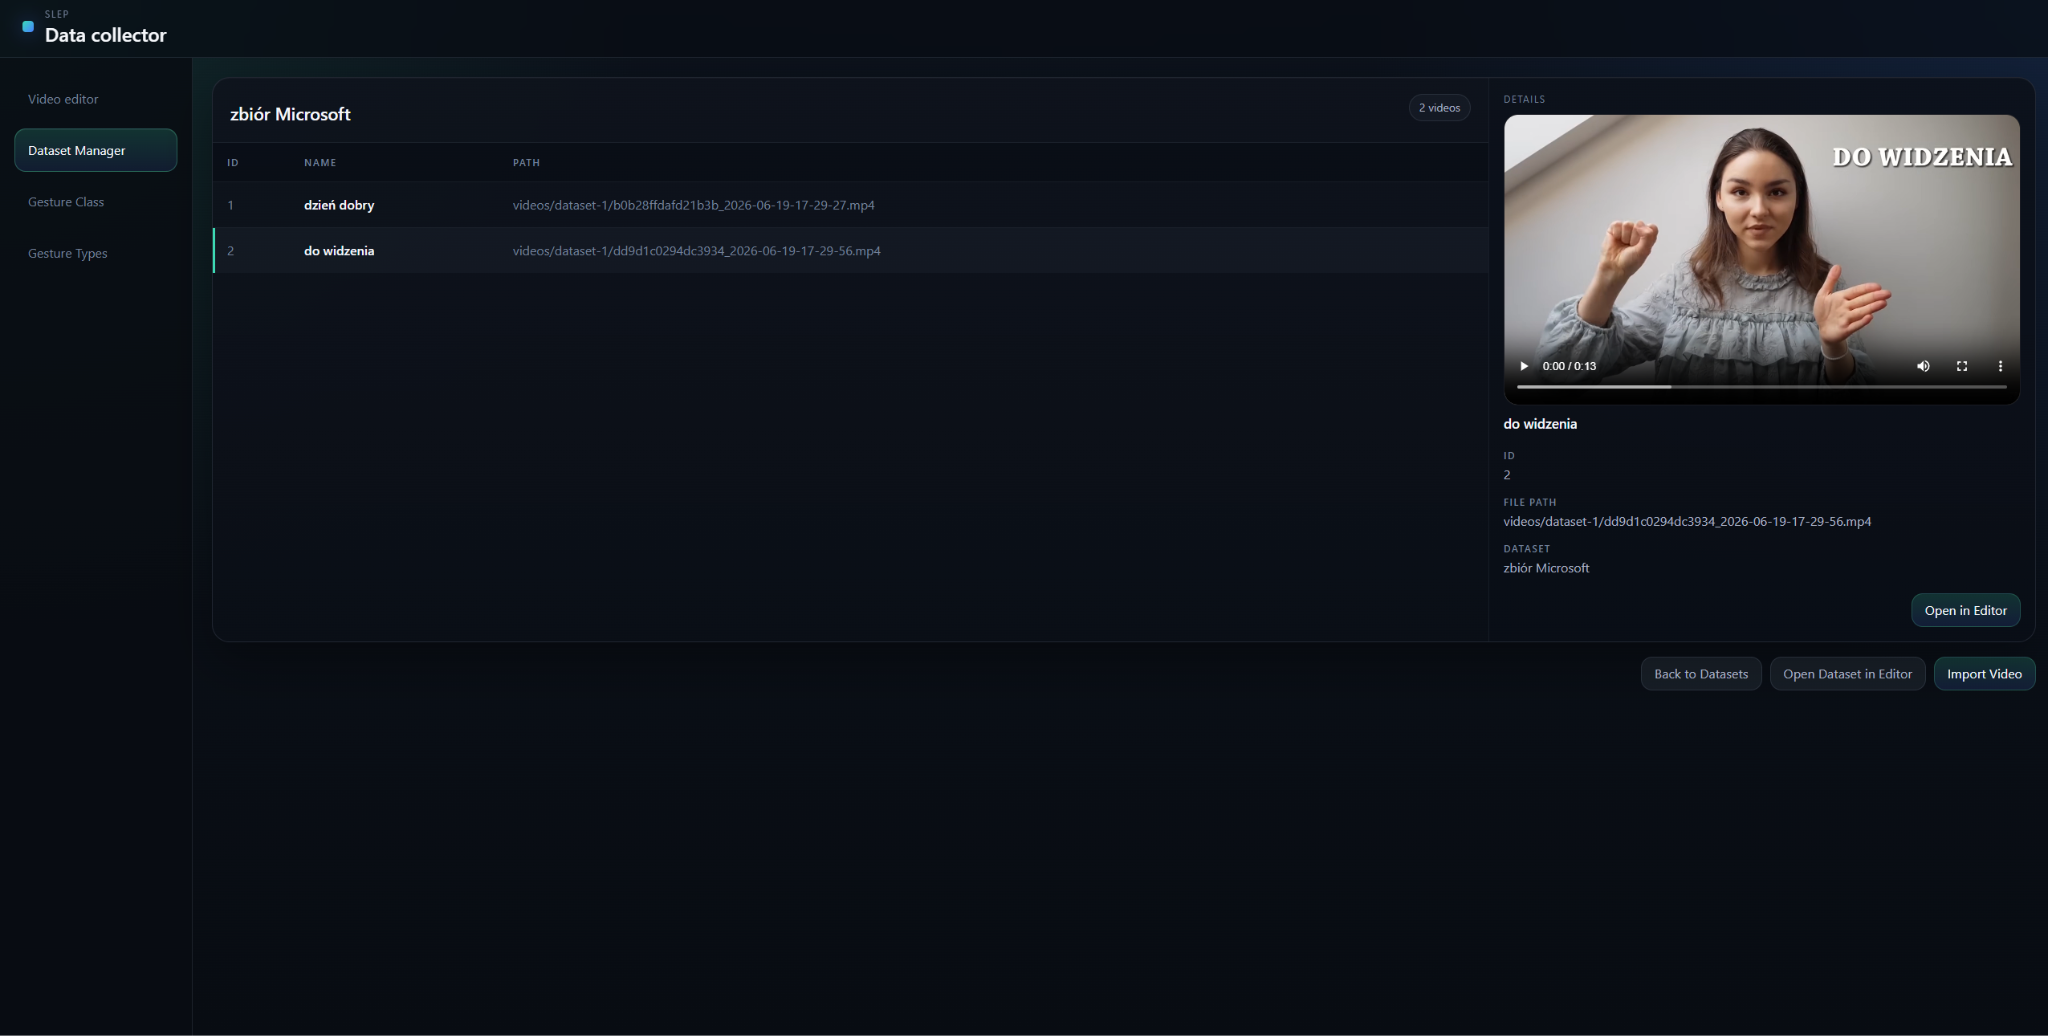
\includegraphics[width=0.85\textwidth]{figures/annotation-platform/dataset-videos-page.png}
  \caption{Widok nagrań w menedżerze zbiorów danych.}
  \label{fig:dataset-videos-page}
\end{figure}

\begin{figure}[htbp]
  \centering
  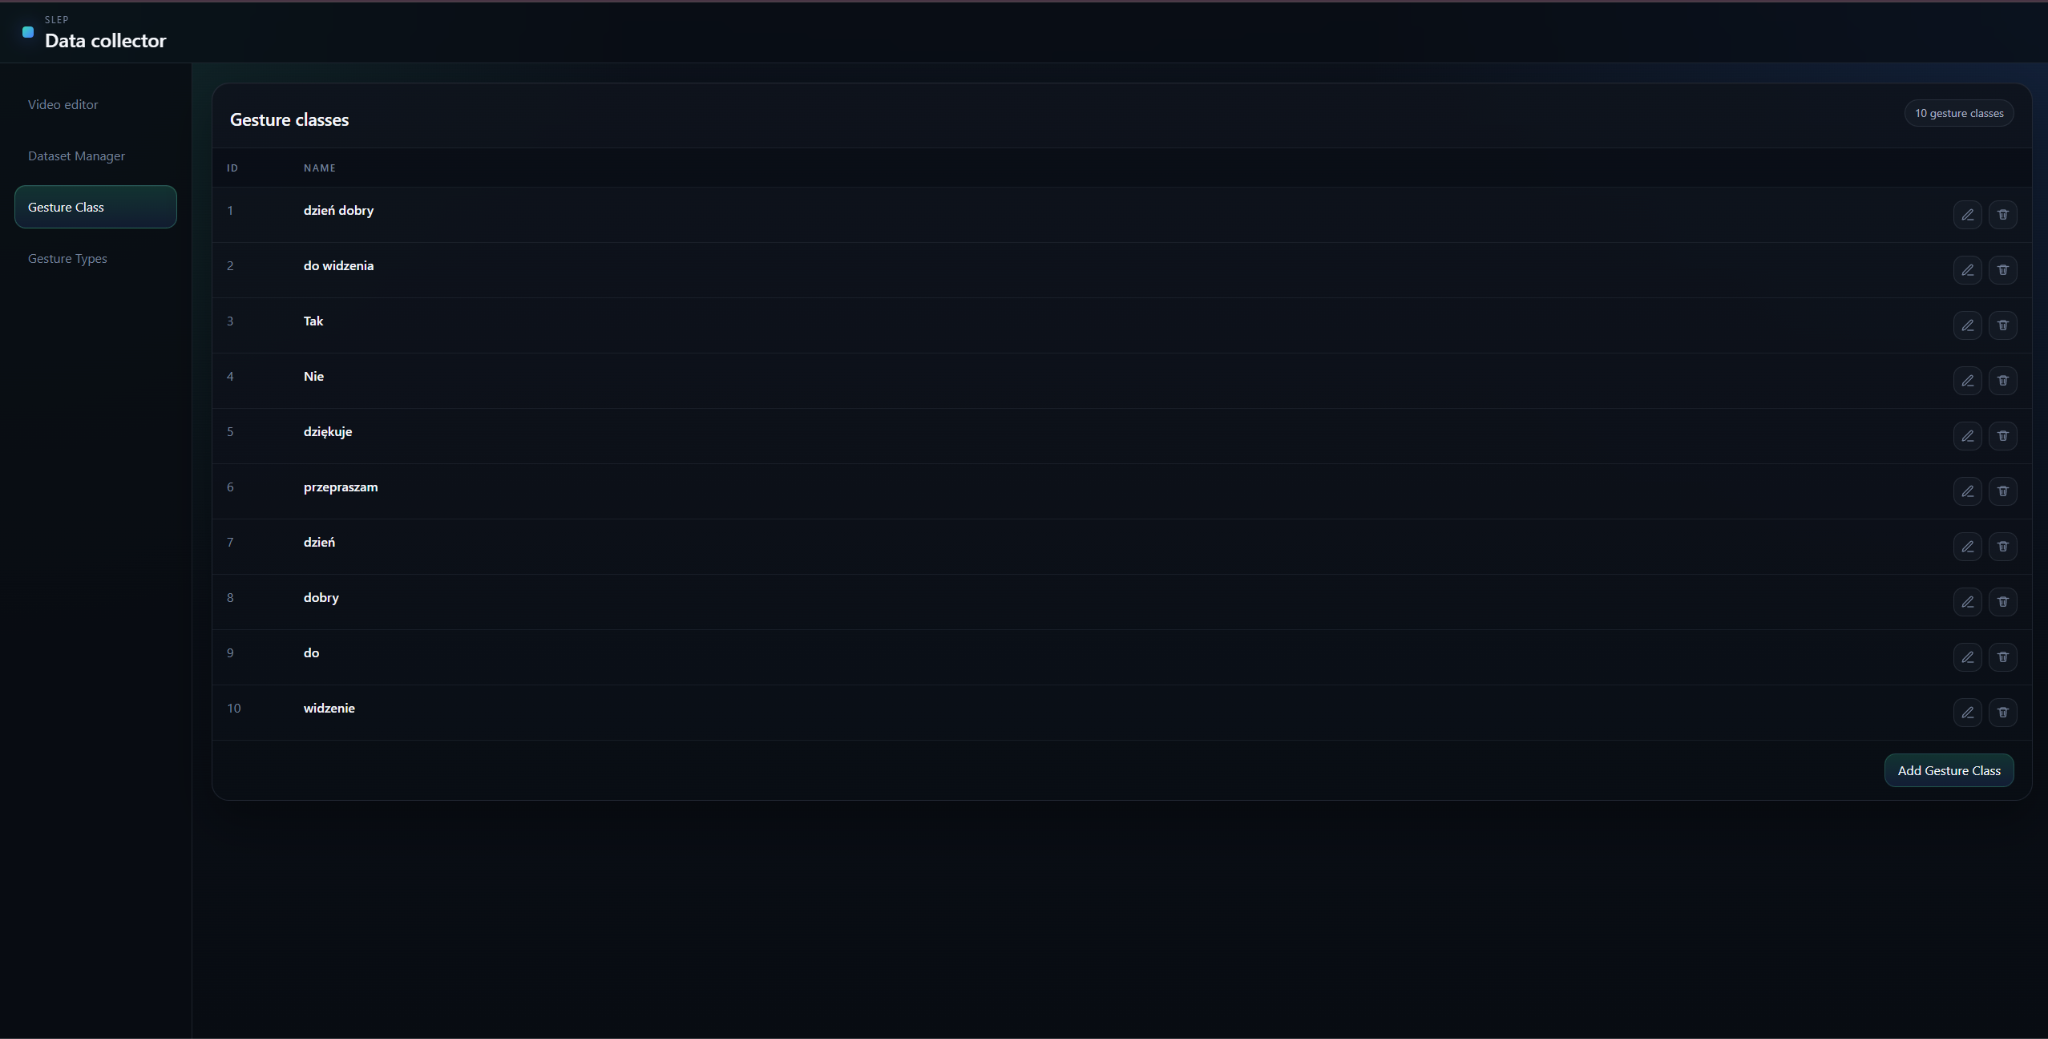
\includegraphics[width=0.7\textwidth]{figures/annotation-platform/gesture-classes-page.png}
  \caption{Widok zarządzania klasami gestów.}
  \label{fig:gesture-classes-page}
\end{figure}

\begin{figure}[htbp]
  \centering
  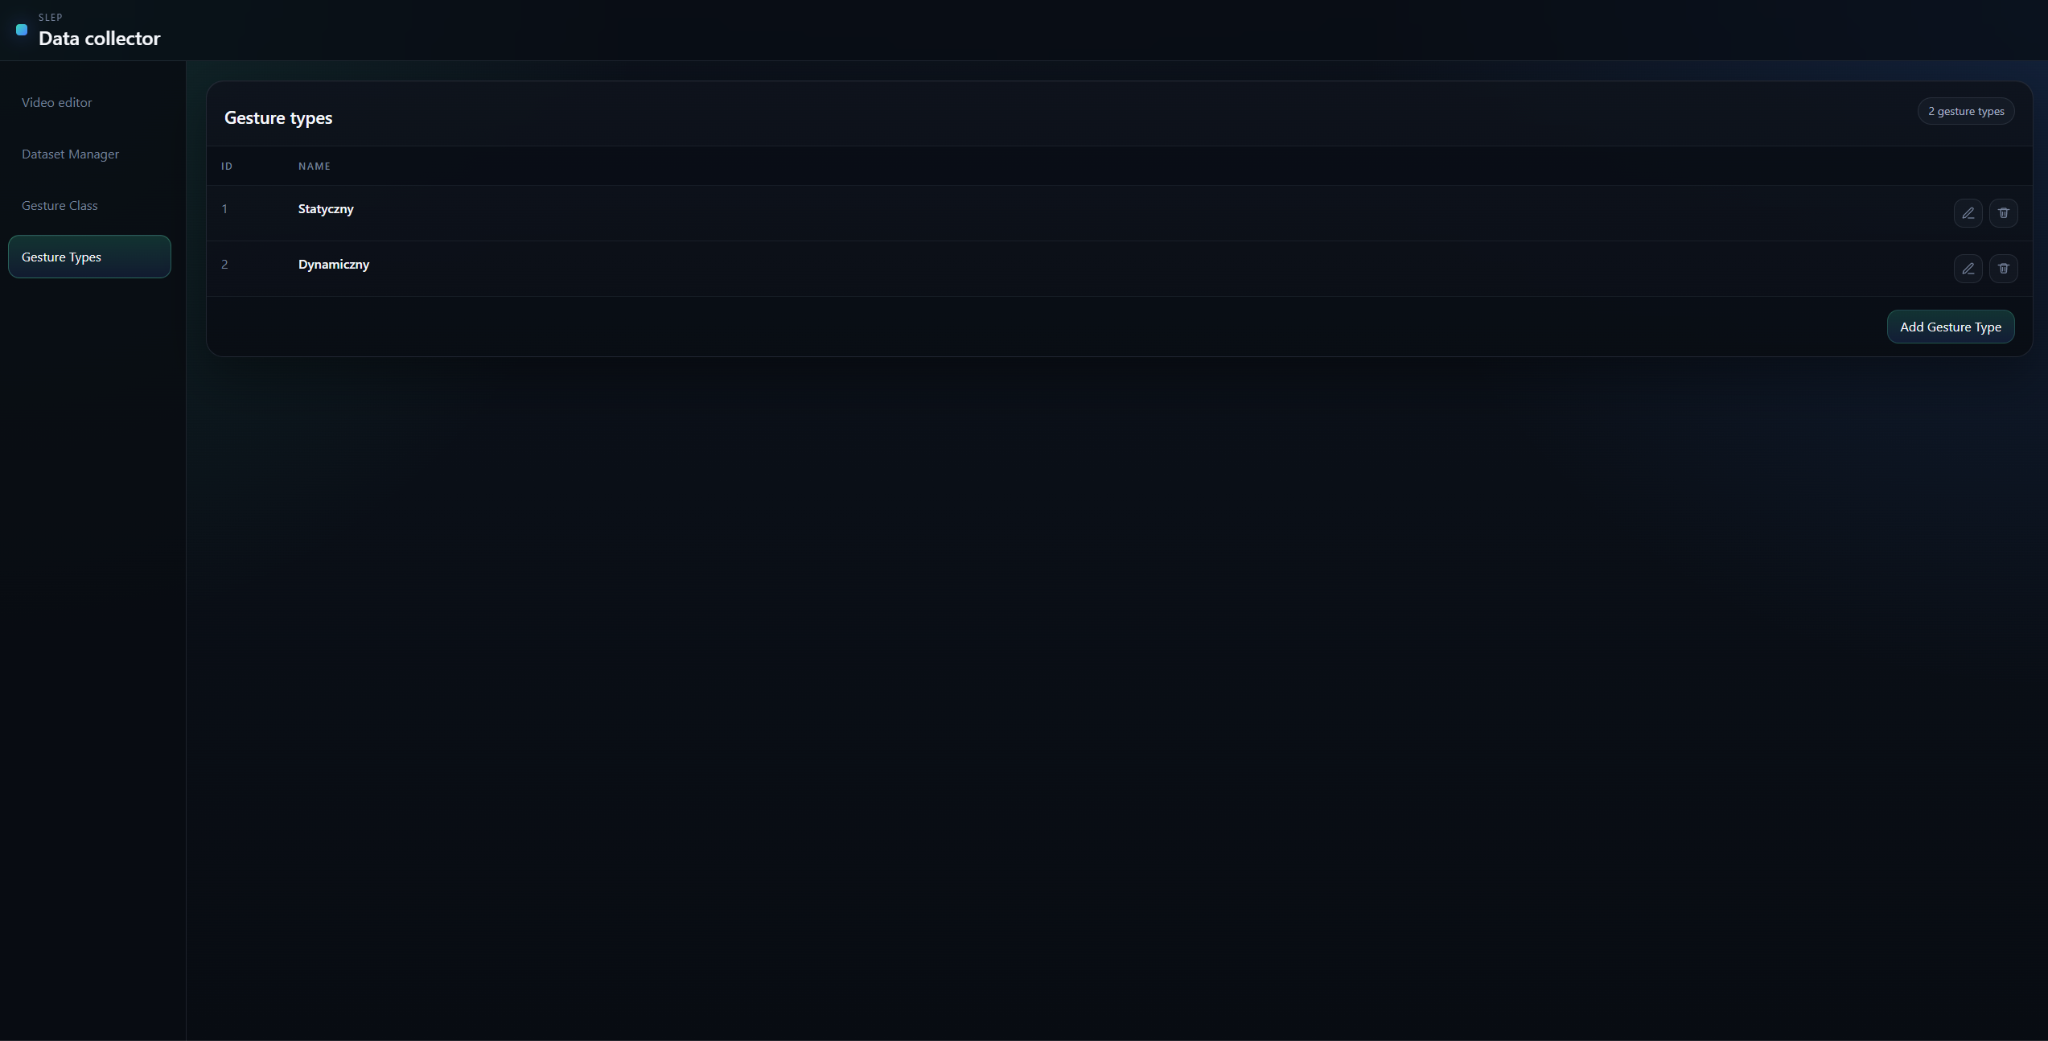
\includegraphics[width=0.7\textwidth]{figures/annotation-platform/gesture-types-page.png}
  \caption{Widok zarządzania typami gestów.}
  \label{fig:gesture-types-page}
\end{figure}

\subsection{Architektura systemu}
\label{sec:annotation-system-architecture}

Aplikacja wykorzystuje typową architekturę full-stack, przedstawioną
na rysunku~\ref{fig:system-architecture}:

\begin{itemize}
  \item frontend w React obsługuje działania użytkownika i komunikuje się
        z backendem za pośrednictwem HTTP;
  \item backend w FastAPI udostępnia endpointy REST dla zbiorów danych, nagrań,
        metadanych gestów, zadań importu, zadań eksportu oraz podpisanych
        adresów URL do S3;
  \item PostgreSQL przechowuje ustrukturyzowane metadane, w tym zbiory danych,
        nagrania, klipy, punkty charakterystyczne, klasy gestów, typy gestów
        i zadania przetwarzania;
  \item MinIO przechowuje duże pliki binarne, takie jak przesłane nagrania
        i wygenerowane tablice punktów charakterystycznych;
  \item Redis pełni funkcję brokera komunikatów dla Celery;
  \item procesy robocze Celery wykonują długotrwałe zadania przetwarzania wideo
        poza cyklem obsługi żądania i odpowiedzi.
\end{itemize}

Rozdzielenie tych zadań jest istotne, ponieważ przetwarzanie wideo może być
kosztowne obliczeniowo. Przesłanie nagrania i zlecenie zadania importu szybko
zwraca sterowanie aplikacji internetowej, podczas gdy ekstrakcja punktów
charakterystycznych jest kontynuowana w procesie roboczym.

\begin{figure}[htbp]
  \centering
  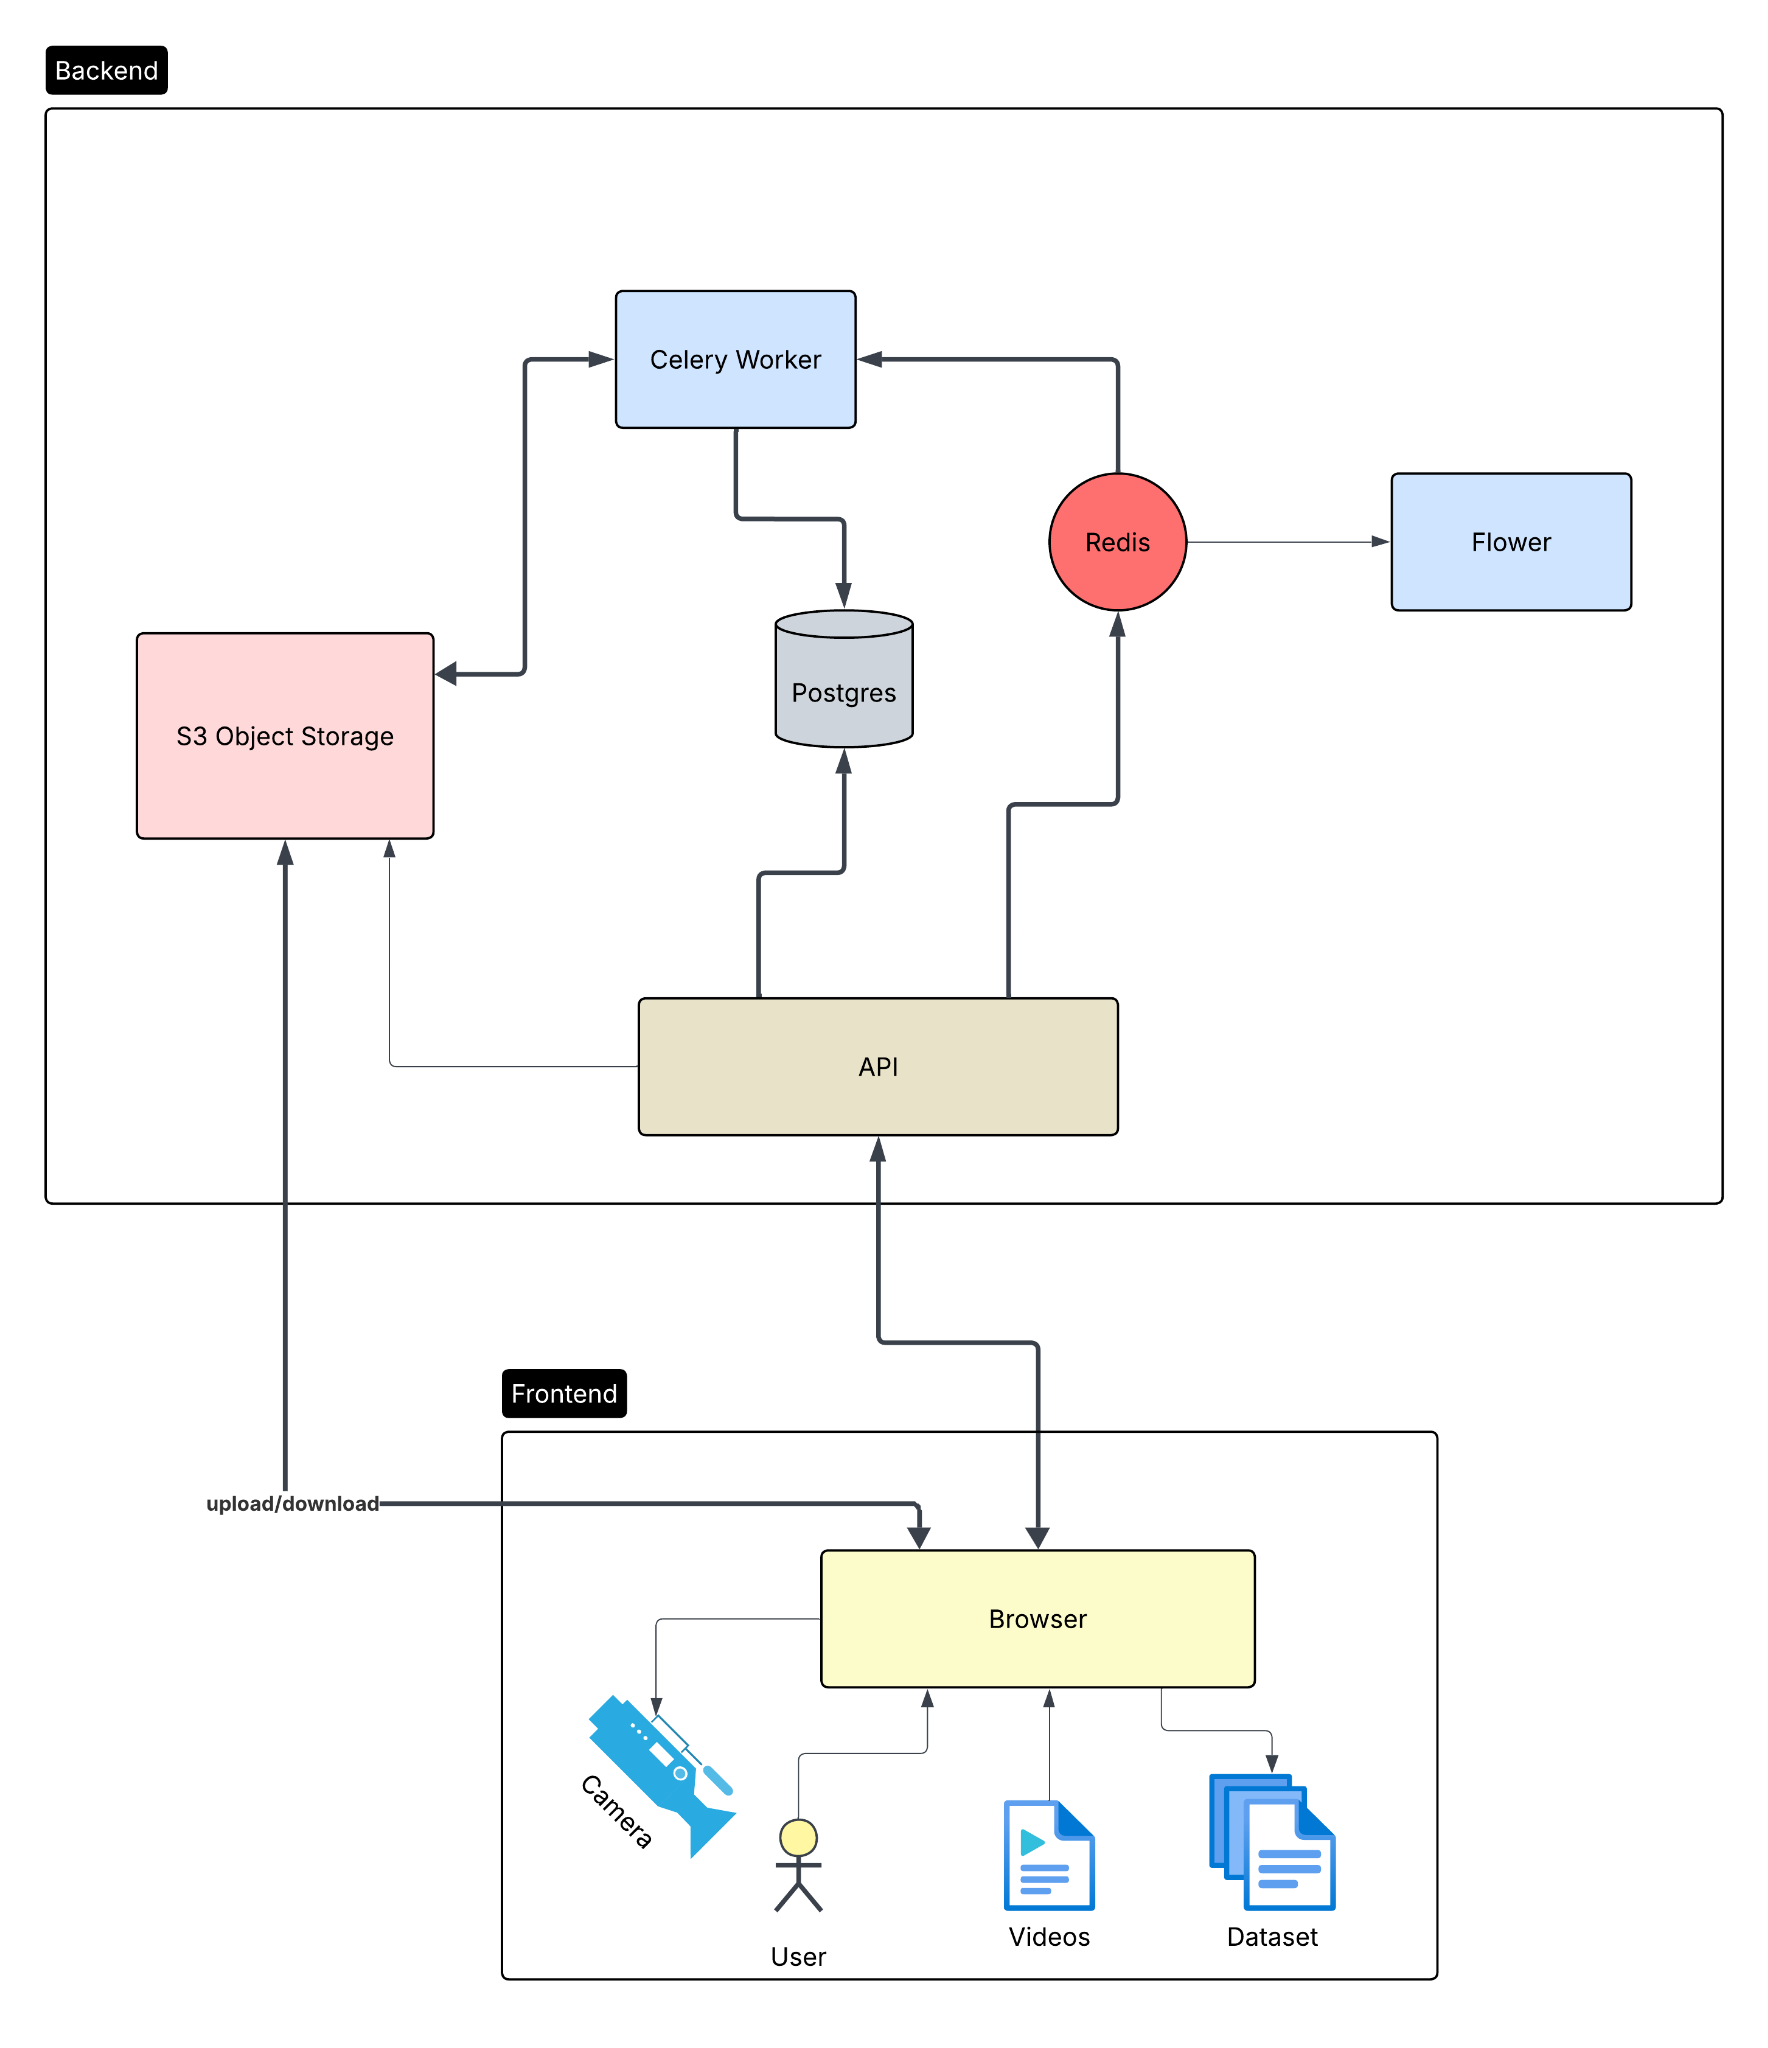
\includegraphics[width=0.85\textwidth]{figures/annotation-platform/system-architecture.png}
  \caption{Schemat architektury systemu platformy do anotacji.}
  \label{fig:system-architecture}
\end{figure}

Backend zaimplementowano przy użyciu Python~3.12, FastAPI, Pydantic,
asynchronicznego SQLAlchemy, Alembic, PostgreSQL, Redis, Celery, MinIO/S3
 i MediaPipe. Udostępnia on endpointy REST pod prefiksem \texttt{/api/v1}
 i wykorzystuje asynchroniczny dostęp do bazy danych podczas obsługi żądań
aplikacji. Jego struktura obejmuje routery API, moduły CRUD, serwisy, schematy
 i modele SQLAlchemy (rysunek~\ref{fig:backend-structure}), a API obejmuje
następujące obszary:

\begin{itemize}
  \item \textbf{zbiory danych}: tworzenie, wyświetlanie listy, odczyt,
        aktualizowanie i usuwanie zbiorów danych;
  \item \textbf{nagrania wideo}: wyświetlanie listy nagrań, filtrowanie według
        zbioru danych, odczyt szczegółów nagrania, aktualizowanie i usuwanie
        nagrań oraz zarządzanie powiązanymi klipami i punktami charakterystycznymi;
  \item \textbf{klasy gestów}: tworzenie, wyświetlanie listy, odczyt,
        aktualizowanie i usuwanie klas gestów;
  \item \textbf{typy gestów}: tworzenie, wyświetlanie listy, odczyt,
        aktualizowanie i usuwanie typów gestów;
  \item \textbf{zadania importu wideo}: tworzenie zadań importu nagrań
        i sprawdzanie ich szczegółów;
  \item \textbf{integracja z S3}: generowanie podpisanych adresów URL
        do przesyłania i pobierania plików;
  \item \textbf{wyeksportowane zbiory danych i zadania eksportu zbiorów danych}:
        struktury bazy danych i API przygotowane z myślą o przyszłej obsłudze
        eksportu zbiorów danych.
\end{itemize}

\begin{figure}[htbp]
  \centering
  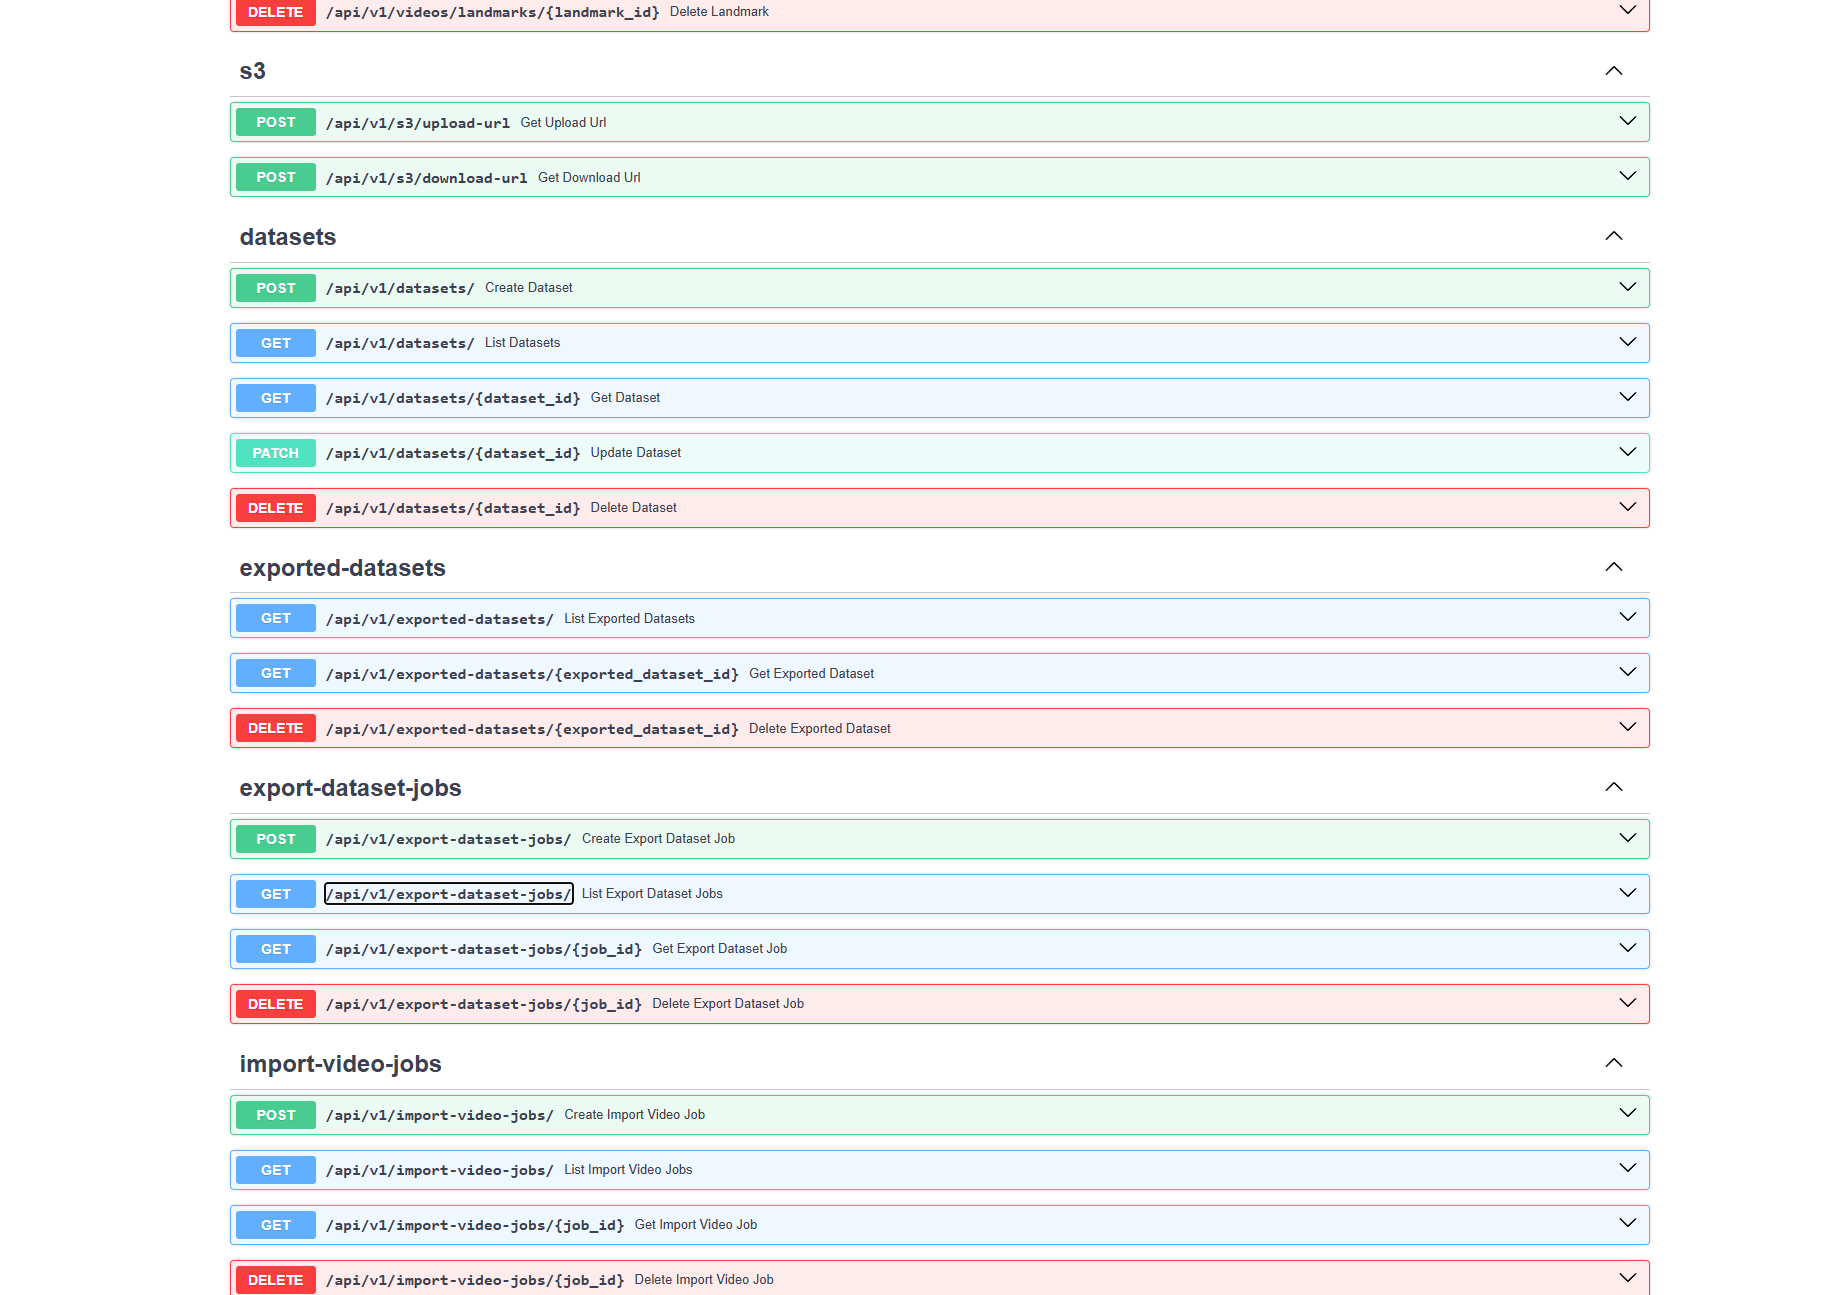
\includegraphics[width=0.7\textwidth]{figures/annotation-platform/swagger-ui.png}
  \caption{API backendu w interfejsie Swagger UI.}
  \label{fig:swagger-ui}
\end{figure}

Proces importu jest obsługiwany przez \texttt{VideoService} oraz zadanie Celery.
Po utworzeniu zadania importu nagrania backend zapisuje metadane zadania i zleca
jego wykonanie w Celery. Proces roboczy pobiera nagranie z MinIO, wyodrębnia
punkty charakterystyczne, zapisuje wynik jako plik NumPy \texttt{.npy}, przesyła go
z powrotem do MinIO, tworzy rekord nagrania i wiąże wygenerowany plik punktów
charakterystycznych z tym nagraniem. Samo przesyłanie pliku odbywa się przy użyciu
podpisanych adresów URL do S3: frontend zwraca się do backendu o adres URL
 do przesyłania, przesyła wybrany plik bezpośrednio do MinIO, a następnie tworzy
zadanie importu odwołujące się do ścieżki przesłanego obiektu. Pozwala to uniknąć
przesyłania dużych plików wideo przez proces aplikacji FastAPI.

Analiza wideo jest wykonywana asynchronicznie przez proces roboczy Celery
(zadanie \texttt{process\_video}). Głównym elementem tego procesu jest
\texttt{LandmarkExtractionService}, który wykorzystuje MediaPipe Holistic firmy
Google i działa w następujący sposób:

\begin{enumerate}
  \item \textbf{Pobranie pliku} -- serwis pobiera plik wideo spod wskazanego
        klucza S3 do lokalnego środowiska procesu roboczego;
  \item \textbf{Inicjalizacja sieci uczenia maszynowego} -- detektor MediaPipe
        Holistic (\texttt{HolisticLandmarker}) jest uruchamiany za pomocą
        menedżera kontekstu;
  \item \textbf{Ekstrakcja na poziomie klatek} -- detekcja jest wykonywana
        dla każdej klatki nagrania w celu wyodrębnienia współrzędnych
        przestrzennych $x$, $y$ i $z$;
  \item \textbf{Wektoryzacja} -- wyniki dla wszystkich komponentów (twarz,
        ciało, dłonie) są łączone w jeden płaski wektor, szczegółowo opisany
        w podrozdziale~\ref{sec:annotation-data-format};
  \item \textbf{Agregacja do macierzy} -- wektory kolejnych klatek są dopisywane
        do listy, która ostatecznie przyjmuje postać dwuwymiarowej macierzy
        o wymiarach [liczba klatek $\times$ liczba cech];
  \item \textbf{Eksport do S3} -- macierz jest serializowana do pliku
        \texttt{.npy} (\texttt{numpy.save()}), a następnie przesyłana do S3;
  \item \textbf{Zapis potwierdzenia w bazie danych} -- w tabeli
        \texttt{landmarks} tworzony jest rekord zawierający klucz S3.
\end{enumerate}

Dla każdej klatki serwis ekstrakcji punktów charakterystycznych zapisuje
współrzędne punktów pozy ciała, twarzy, lewej dłoni i prawej dłoni w wierszu
 o stałym rozmiarze. Brakujące detekcje są reprezentowane przez zera, co zapewnia
jednakowe wymiary tablicy wynikowej dla wszystkich klatek i upraszcza jej
późniejsze wykorzystanie w uczeniu maszynowym
(rysunek~\ref{fig:annotation-methodology}).

\begin{figure}[htbp]
  \centering
  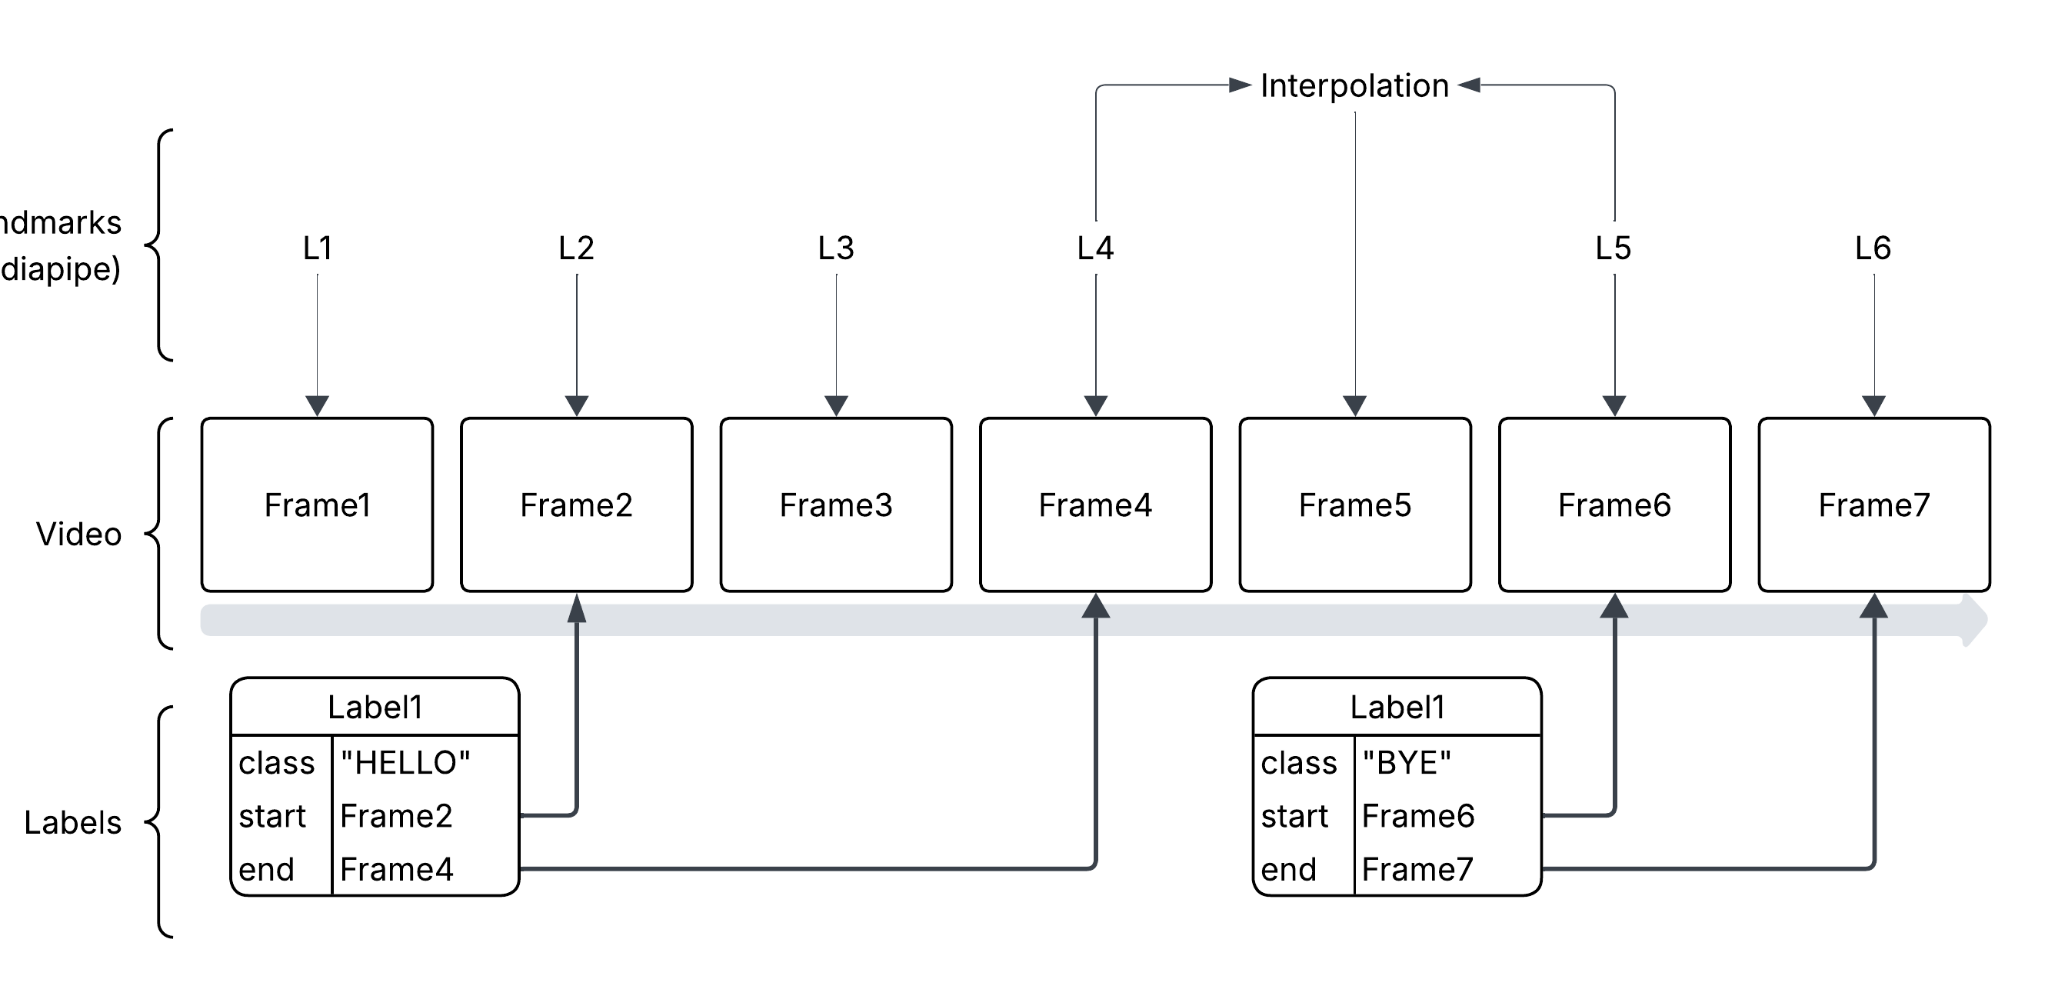
\includegraphics[width=0.85\textwidth]{figures/annotation-platform/annotation-methodology.png}
  \caption{Metodyka anotacji nagrań wideo za pomocą glos.}
  \label{fig:annotation-methodology}
\end{figure}

Obecny model bazy danych obejmuje następujące główne encje:

\begin{itemize}
  \item \textbf{Dataset} -- nazwany zbiór powiązanych nagrań;
  \item \textbf{Video} -- metadane przechowywanego nagrania, w tym ścieżka
        pliku, opis, liczba klatek na sekundę (FPS), czas trwania i powiązanie
        ze zbiorem danych;
  \item \textbf{Landmark} -- metadane wygenerowanych plików punktów
        charakterystycznych powiązanych z nagraniami;
  \item \textbf{Clip} -- anotowany zakres klatek w obrębie nagrania;
  \item \textbf{GestureClass} -- kategoria etykiety przypisywanej klipom;
  \item \textbf{GestureType} -- dodatkowa klasyfikacja gestów przypisywana klipom;
  \item \textbf{ImportVideoJob} -- stan przetwarzania importu nagrania
        i ekstrakcji punktów charakterystycznych;
  \item \textbf{ExportDatasetJob} -- stan przetwarzania przyszłych zadań
        eksportu zbiorów danych;
  \item \textbf{ExportedDataset} -- metadane opisujące wygenerowane,
        wyeksportowane zbiory danych.
\end{itemize}

Powiązania między nagraniami, klipami, punktami charakterystycznymi, klasami
 i typami gestów tworzą ustrukturyzowaną warstwę anotacji surowych danych wideo,
przydatną do późniejszego eksportu zbiorów danych i przygotowania ich do
trenowania modeli. Kluczowe decyzje architektoniczne dotyczące modelu danych
obejmują:

\begin{itemize}
  \item stosowanie \texttt{ON DELETE CASCADE} dla powiązanych rekordów
        (np.\ klipów, punktów charakterystycznych i zadań eksportu zbiorów danych)
        po usunięciu encji nadrzędnej, co eliminuje osierocone dane;
  \item stosowanie \texttt{ON DELETE SET NULL} w relacji zbiorów danych
        z nagraniami: usunięcie zbioru danych nie usuwa jego nagrań, lecz jedynie
        ustawia \texttt{dataset\_id} na \texttt{NULL}, zachowując cenne dane wideo;
  \item typy \texttt{ENUM} dla statusów zadań (\texttt{in\_queue},
        \texttt{processing}, \texttt{done}, \texttt{error}), wymuszające spójność
        danych;
  \item denormalizację w \texttt{exported\_datasets}: nazwa i opis zbioru danych
        są kopiowane w momencie eksportu, dzięki czemu migawka pozostaje
        niezmienna, a historyczny stan zbioru można zawsze odtworzyć;
  \item oddzielenie logiki przetwarzania (\texttt{import\_video\_jobs},
        \texttt{export\_dataset\_jobs}) od danych biznesowych (nagrań, klipów
        i punktów charakterystycznych);
  \item rozdzielenie semantyki gestów na \texttt{gesture\_classes} (ogólne
        kategorie) i \texttt{gesture\_types} (konkretne typy), co umożliwia
        bardziej elastyczne modelowanie danych;
  \item dopuszczenie wartości null w polach zadań (\texttt{video\_id},
        \texttt{error\_message}, \texttt{dataset\_id},
        \texttt{exported\_dataset\_id}), umożliwiające stopniowe uzupełnianie
        rekordów podczas przetwarzania;
  \item brak mechanizmu usuwania logicznego: usunięcie encji jest operacją
        fizyczną i nieodwracalną.
\end{itemize}

Projekt zawiera usługi Docker Compose tworzące kompletne środowisko
programistyczne: \texttt{postgres} do przechowywania metadanych w relacyjnej
bazie danych, \texttt{redis} do komunikacji z kolejką Celery,
\texttt{s3-dev}/\texttt{s3} jako magazyn obiektowy MinIO,
\texttt{data-collection-api} jako backend FastAPI,
\texttt{data-collection-worker} do przetwarzania w tle przez Celery,
\texttt{data-collection-flower} do monitorowania procesów roboczych Celery oraz
\texttt{data-collection-frontend} do udostępniania zbudowanego frontendu przez
Nginx. Frontend przechowuje typy API i funkcje wysyłające żądania we wspólnym
module akcji, podczas gdy strony i komponenty koncentrują się na obsłudze działań
użytkownika (rysunek~\ref{fig:frontend-structure}). Backend rozdziela routery,
schematy, operacje CRUD, serwisy, modele i zadania procesów roboczych
(rysunek~\ref{fig:backend-structure}). Zmiany schematu bazy danych są obsługiwane
za pomocą migracji Alembic.

\begin{figure}[htbp]
  \centering
  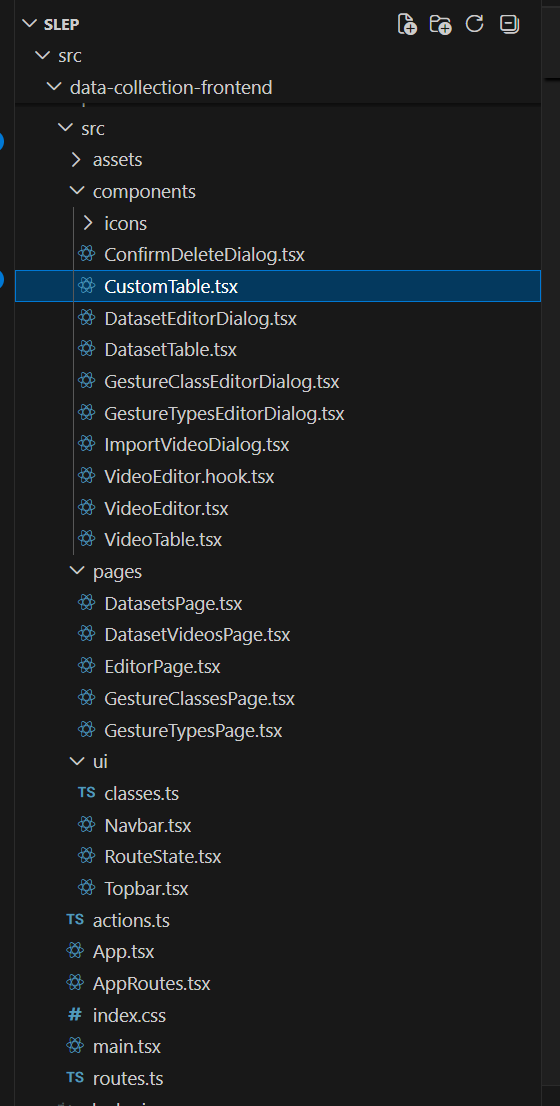
\includegraphics[width=0.6\textwidth]{figures/annotation-platform/frontend-structure.png}
  \caption{Struktura projektu frontendu.}
  \label{fig:frontend-structure}
\end{figure}

\begin{figure}[htbp]
  \centering
  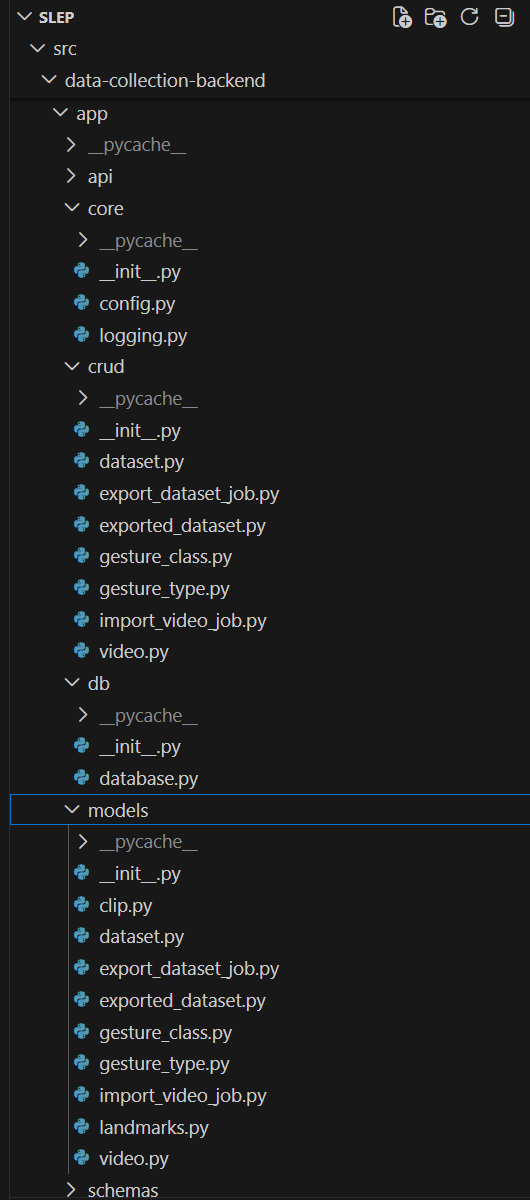
\includegraphics[width=0.5\textwidth]{figures/annotation-platform/backend-structure.png}
  \caption{Struktura projektu backendu.}
  \label{fig:backend-structure}
\end{figure}

\subsection{Format i struktura danych}
\label{sec:annotation-data-format}

Pliki punktów charakterystycznych są przechowywane w Amazon S3 jako binarne
macierze NumPy (\texttt{.npy}). Nagrania są identyfikowane przez dowolny klucz S3,
 a odpowiadający im plik punktów charakterystycznych wykorzystuje ten sam klucz
z przyrostkiem \texttt{\_landmarks.npy}. Każdy plik \texttt{.npy} zawiera
macierz dwuwymiarową o wymiarach [liczba klatek nagrania] $\times$ [1659],
zgodnie z zestawieniem w tabeli~\ref{tab:landmark-vector}.

\begin{table}[htbp]
  \centering
  \caption{Struktura wektora cech punktów charakterystycznych dla pojedynczej klatki (1659 wartości).}
  \label{tab:landmark-vector}
  \begin{tabular}{lccc}
    \hline
    \textbf{Komponent} & \textbf{Zakres indeksów} & \textbf{Punkty} & \textbf{Wartości ($x,y,z$)} \\
    \hline
    Poza (sylwetka) & 0--98    & 33  & 99   \\
    Twarz           & 99--1532 & 478 & 1434 \\
    Lewa dłoń       & 1533--1595 & 21 & 63  \\
    Prawa dłoń      & 1596--1658 & 21 & 63  \\
    \hline
    \textbf{Łącznie} & --       & 553 & 1659 \\
    \hline
  \end{tabular}
\end{table}

Jeśli dany element nie zostanie wykryty w danej klatce (np.\ brak detekcji prawej
dłoni), wszystkie przypisane mu wartości są ustawiane na $0.0$. Wynikowa
reprezentacja -- jeden wiersz na klatkę nagrania, 1659 kolumn typu float32
w każdym wierszu -- jest tą samą reprezentacją punktów charakterystycznych,
którą wykorzystuje potok przetwarzania wstępnego modelu rozpoznawania izolowanych
glos, opisany w podrozdziale~\ref{sec:gloss-recognition-preprocessing}.

Całościowy przepływ danych przez platformę przebiega w trzech etapach:

\begin{enumerate}
  \item \textbf{Import nagrania} -- w \texttt{import\_video\_jobs} tworzony jest
        rekord ze statusem \texttt{in\_queue}; status jest zmieniany na
        \texttt{processing}; plik zostaje pobrany i odczytywane są jego metadane
        (FPS, czas trwania); tworzony jest rekord w \texttt{videos}; na końcu
        status zadania jest zmieniany na \texttt{done} (z uzupełnionym
        \texttt{video\_id}) lub \texttt{error} (z uzupełnionym
        \texttt{error\_message});
  \item \textbf{Przetwarzanie nagrania (ekstrakcja punktów charakterystycznych)}
        -- proces roboczy Celery pobiera nagranie z S3, uruchamia MediaPipe
        Holistic dla każdej klatki, generuje macierz punktów charakterystycznych
        i zapisuje ją w S3, tworzy rekord w \texttt{landmarks} oraz rekordy
        w \texttt{clips} z przypisanymi \texttt{gesture\_class\_id}
        i \texttt{gesture\_type\_id};
  \item \textbf{Eksport zbioru danych} -- w \texttt{export\_dataset\_jobs}
        tworzony jest rekord ze statusem \texttt{in\_queue}; proces roboczy
        generuje pakiet danych (nagrania i punkty charakterystyczne) dla
        wszystkich nagrań w zbiorze; tworzony jest rekord
        w \texttt{exported\_datasets} (ze zdenormalizowanymi danymi zbioru);
        status zadania jest zmieniany na \texttt{done} lub \texttt{error}.
\end{enumerate}

Na obecnym etapie projekt zapewnia działającą podstawę do zarządzania zbiorami
nagrań wideo i ich anotacji, obsługując pełną ścieżkę od utworzenia zbioru danych,
przez przesłanie nagrania, po ekstrakcję punktów charakterystycznych w tle
 i anotację klipów. Najbardziej rozwinięte obszary to struktura operacji CRUD
 i API REST backendu, lokalna orkiestracja usług za pomocą Docker Compose,
przesyłanie nagrań zgodne z S3, asynchroniczna ekstrakcja punktów
charakterystycznych przez Celery, zarządzanie zbiorami danych i taksonomią gestów
w interfejsie użytkownika oraz anotacja klipów na osi czasu w przeglądarce.
Obsługa eksportu zbiorów danych obejmuje modele bazy danych, schematy, moduły CRUD
 i endpointy API, jednak asynchroniczny potok przetwarzania eksportu nadal wymaga
ukończenia, a aktualizacje statusu zadań importu powinny być bardziej jednoznacznie
realizowane w całym cyklu działania procesu roboczego.

Do znanych ograniczeń obecnej platformy należą: metadane nagrań, takie jak FPS
 i czas trwania, są obecnie zapisywane w procesie roboczym jako stałe wartości,
zamiast być w pełni wyznaczane na podstawie przesłanego pliku; bazowy adres URL
API we frontendzie jest zapisany na stałe, zamiast podlegać konfiguracji;
uwierzytelnianie i autoryzacja nie zostały zaimplementowane; walidacja zakresów
klipów, zduplikowanych etykiet i spójności zbiorów danych może zostać rozszerzona;
generowanie podglądów punktów charakterystycznych zostało uwzględnione w modelu,
ale nie jest w pełni zaimplementowane. Zakres automatycznych testów jest również
ograniczony. Najważniejsze obszary przyszłych testów obejmują zachowanie
endpointów API, działanie procesów roboczych przy udanych i nieudanych importach,
walidację migracji bazy danych, zachowanie edytora we frontendzie podczas wyboru
klatek i zapisywania klipów oraz testy integracyjne pełnej ścieżki przesyłania,
importu i przetwarzania. Ograniczenia te nie uniemożliwiają lokalnych eksperymentów
z gromadzeniem danych, ale powinny zostać usunięte przed wykorzystaniem platformy
jako niezawodnego narzędzia do obsługi danych produkcyjnych lub badawczych.

\todo{DO UZUPEŁNIENIA: Należy wstawić diagram związków encji przedstawiający
schemat tabel \texttt{datasets} / \texttt{videos} / \texttt{clips} /
\texttt{landmarks} / \texttt{gesture\_classes} / \texttt{gesture\_types} /
\texttt{import\_video\_jobs} / \texttt{export\_dataset\_jobs} /
\texttt{exported\_datasets} oraz powiązania między nimi za pomocą kluczy obcych.}